% Appendix H: the binding swap of Prakash et al. Input by sections/appendix.tex.
\section{The binding swap of Prakash et al.}\label{app:binding}\label{sec:prakash}

Preregistration H applied the key-only and value-only exchange to an edit we did not design: the state-token patch BIND of \citet{prakash2025lookbacks}, at Qwen2.5-14B on their material, with an identity edit ID as a control. Its four predictions on the swap (H7--H10) failed. The final round asked two narrower questions on the same material: whether an identity edit is copy-read at the swap's depth (J-C6), and whether any model has a depth at which the binding swap works while the identity key route is still open, the only depth at which the two kinds of edit could be compared (the overlap screen). \Cref{tab:prereg-h} gives the verdicts of H, and \cref{app:prereg-j} those of the final round.

\subsection{The exchange at Qwen2.5-14B (preregistration H, part (b))}\label{app:prakash}

BIND replicates (IIA \PkGatebOneBind{} at block \PkLstar{} under \fmtNone{}; Gate b1).

\paragraph{The binding swap is key-dominant; four predictions failed.}
Without a later mention, keys carry most of BIND's effect and values a substantial share ($\psi_K = \PkPsiKBindNone{}$, $\psi_V = \PkPsiVBindNone{}$, $\kappa = \PkKappaBindNone{}$). Under \textsc{qnames} and \fmtOpt{}, $\kappa = \PkKappaBindQnames{}$ and \PkKappaBindOpt{}, but BIND flips \PkNflipBindQnames{}/\PkN{} answers there (exploratory count), so these decompose a shift of the logit margin; \fmtLetter{} failed the effect-size gate. Not met: values carrying BIND without a later mention (H8); a crossover of at least 0.4 (later mentions raised $\kappa$ by \HnineDiff{} [\HnineDiffLo{}, \HnineDiffHi{}], and \textsc{qnames} is not in between; H9); the rival $\kappa \leq 0.25$ (H10; nor is $\kappa \geq 0.75$ throughout); and the law $\kappa \approx s_{\mathrm{ID}}$, which missed by \HsevenGapMin{}--\HsevenGapMax{} (H7; \cref{fig:frames}c).

\paragraph{The identity edit, and depth.}
ID at block 0 matched the law ($\kappa_{\mathrm{ID}}$ = \PkKappaIdZeroNone{}, \PkKappaIdZeroQnames{}, \PkKappaIdZeroOpt{} against $s_{\mathrm{ID}}$ = \HelevenSidNone{}, \HelevenSidQnames{}, \HelevenSidOpt{}), and later mentions raised $\kappa_{\mathrm{ID}}$ by \HelevenDiff{} [\HelevenDiffLo{}, \HelevenDiffHi{}] (H11, met). This is consistency on their material, not out-of-sample support: at block 0 ID nearly equals the natural clamp, and H11's block-28 part compares values near zero. Post hoc, at block 28 BIND is key-dominant while ID is value-carried ($\psi_V \geq \PkPsiVIdTwentyeightOpt{}$ in the evaluable formats), which is consistent with the H7 failure but does not explain it. Depth is an alternative explanation (below): no depth has both the binding swap and a key-read identity route, so whether the kind of edit or its depth sets how far the format moves the attribution is untested.

\paragraph{Material and population.} We use the template-2 stories of \citet{prakash2025lookbacks}, their raw prompt (an instruction, the story, ``Question:'' and ``Answer:'', without a chat template) and their pool of \PkNpool{} reversed-sentence pairs drawn with their seed. In each story two characters each fill an opaque bottle with a drink, in two sentences, and the question asks what one character believes their bottle contains. The release is fetched at run time and checked by hash, and our port reproduces their pool byte for byte. Their language-model filter under \fmtNone{} passed \PkNpass{} pairs at Qwen2.5-14B-Instruct; the population is the first \PkN{} passing pairs in pool order, of which about \PkOverlap{} are in their 80-pair validation split. The formats differ only after the story: \fmtNone{} is their question; \textsc{qnames} names four candidate drinks in the question (the two story drinks and two drinks S and X absent from the story); \fmtOpt{} lists the same four as choices with ``Answer with exactly one choice''; \fmtLetter{} letters them (exploratory); and \textsc{qnames2} (exploratory) names only the two story drinks, as the questions of their preliminary second dataset do.

\paragraph{The two edits.} BIND is their state-token patch: at the output of block $\ell^*$, the residuals at the two drink words and the punctuation after each are set to those of the counterfactual in which the two sentences are exchanged, each position taking the other sentence's. The drink words' identity does not change; their ordering information does. These are the ordering IDs on which the binding, answer and visibility lookbacks of \citet{prakash2025lookbacks} are built, so the swap is not an identity edit. ID substitutes, at block $\ell^*_{\mathrm{ID}}$, the queried drink's span from a donor story in which that drink is replaced by S. With $m = \log p(\text{target}) - \log p(\text{queried drink})$, where the target is the other story drink for BIND and S for ID, IIA is the fraction of pairs whose patched answer is the target, and $\ell^*$ and $\ell^*_{\mathrm{ID}}$ are the earliest blocks whose IIA under \fmtNone{} is within 0.01 of the maximum.

\begin{table}[!ht]
\centering
\small
\caption{\textbf{Replication of the binding swap} (Qwen2.5-14B-Instruct, \fmtNone{}, IIA of BIND by patched block). Released: the per-layer values published with \citet{prakash2025lookbacks} on their 80 validation pairs, transcribed from their release (not part of our results). Ours: \PkN{} pairs, and the \PkSharedN{} pairs shared with their validation split (exploratory). Recomputed from our sweep files; a reproduction check, since the released values were seen before preregistration H was finalised.}
\label{tab:replication}
\begin{tabular}{@{}lccc@{}}
\toprule
Block & Prakash et al.\ (80 pairs) & ours (150 pairs) & ours, 70 shared pairs \\
\midrule
24 & 0.69 & 0.720 & 0.700 \\
26 & 0.72 & 0.747 & 0.729 \\
28 & 1.00 & 0.993 & 1.000 \\
30--34 & 1.00 & 1.000 & 1.000 \\
36 & 0.06 & 0.080 & 0.057 \\
\bottomrule
\end{tabular}

\end{table}

\paragraph{Replication and sweeps.} The swap reproduces their released per-layer IIA (\cref{tab:replication}). Its IIA is 1.00 at blocks 29--34 and \PkGatebOneBind{} at 28, where one pair fails; the tie rule selects $\ell^* = \PkLstar{}$, and one more failure would have selected 29. Below block 24 it flips no answer under \fmtNone{} (IIA \PkSweepIIABindNoneTwentythree{} at block 23, \PkSweepIIABindNoneTwentyfour{} at 24). \Cref{fig:sweeps} shows every sweep. The swap reproduces only under \fmtNone{}: under \textsc{qnames}, \fmtOpt{} and \fmtLetter{} its IIA is at most \PkSweepIIABindQnamesTwentythree{} at every swept block from 18 to 40, and its effect on the margin peaks at \PkSweepPhiBindOptTwentyeight{} nats (\fmtOpt{}, block 28), \PkSweepPhiBindQnamesThirtyone{} (\textsc{qnames}, block 31) and \PkSweepPhiBindLetterTwentythree{} (\fmtLetter{}, block 23). The identity edit flips every answer under \fmtNone{} at every block through 35, so its curve is flat and the tie rule picks $\ell^*_{\mathrm{ID}} = \PkLstarId{}$ by default rather than by localisation. When the candidates are named after the question it stops flipping answers from about block 20: under \fmtOpt{} its IIA is \PkSweepIIAIdOptEleven{} through block 11, \PkSweepIIAIdOptFourteen{} at 14, \PkSweepIIAIdOptSixteen{} at 16, \PkSweepIIAIdOptNineteen{} at 19 and \PkSweepIIAIdOptTwenty{} from 20; under \textsc{qnames} it is \PkSweepIIAIdQnamesZero{} at block 0 and \PkSweepIIAIdQnamesTwenty{} from 20.

\begin{figure}[!ht]
\centering
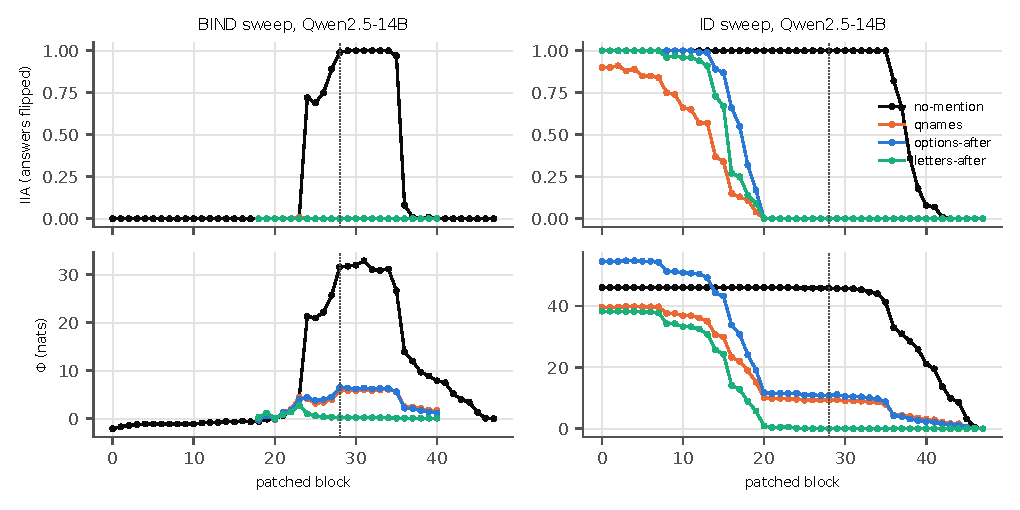
\includegraphics[width=\textwidth]{figures/fig_sweeps.pdf}
\caption{\textbf{Sweeps of the two edits over the patched block} (Qwen2.5-14B-Instruct, \PkN{} pairs, BF16). Top: IIA, the fraction of answers flipped to the target; bottom: $\Phi$, the mean shift of $m = \log p(\text{target}) - \log p(\text{queried drink})$. Left: the binding swap BIND (swept over blocks 18--40 in the formats that name candidates); right: the identity edit ID. Dotted: block $\ell^* = \PkLstar{}$. $\ell^*$ and $\ell^*_{\mathrm{ID}}$ are chosen on the \fmtNone{} sweeps (preregistered); the other formats are reported.}
\label{fig:sweeps}
\end{figure}

\paragraph{The exchange.} The exchange (\cref{app:impl}) exchanges the patched positions' keys or values in every block after the patched one. A cell is evaluable if Gates b0 and b2 pass in it ($\Phi \geq 3$ nats), $\psi_K + \psi_V \geq 0.5$ with both at least $-0.1$, and the edit reproduces at that depth on the \fmtNone{} sweep. \Cref{tab:prakash} summarises the cells and \cref{tab:exchange} gives all thirteen. \fmtLetter{} fails Gate b2 at block 28 for both edits ($\Phi$ = \PkPhiBindLetter{} and \PkPhiIdTwentyeightLetter{} nats), and ID@28 under \fmtLetter{} also fails the $\kappa$ rule; \fmtLetter{} is exploratory throughout. BIND reproduces fully under \fmtNone{} (it flips \PkNflipBindNone{} of \PkN{} answers; exploratory count), and that cell carries H8 by itself. Under \textsc{qnames} and \fmtOpt{} it flips \PkNflipBindQnames{} and \PkNflipBindOpt{} answers, so those cells decompose a shift of the logit margin ($\Phi$ = \PkPhiBindQnames{} and \PkPhiBindOpt{} nats against base margins of $\PkMarginBindQnames$ and $\PkMarginBindOpt$, exploratory, recomputed), not a reproduced swap.

\begin{table}[!ht]
\centering
\caption{\textbf{The exchange on the interventions of \citet{prakash2025lookbacks}} (Qwen2.5-14B-Instruct, \PkN{} pairs). Each cell: $\kappa = \psi_K/(\psi_K+\psi_V)$ with ($\psi_K$, $\psi_V$), the number of answers the full patch flips, and its effect $\Phi$ on the margin (nats). BIND@28: the binding swap at block $\ell^* = \PkLstar{}$; ID@0, ID@28: the identity edit at blocks 0 and 28. $s_{\mathrm{ID}}(f, \ell_0)$: identity key share of the natural clamp at the queried drink from block $\ell_0$, with 95\% CI. $^\dagger$Exploratory formats. $^\ddagger$Gate b2 failed ($\Phi < 3$ nats). n/e: the $\kappa$ rule fails. H7 compares BIND@28 with $s_{\mathrm{ID}}(f, 29)$, H11 ID@0 with $s_{\mathrm{ID}}(f, 1)$ (Part 1) and ID@28 with $s_{\mathrm{ID}}(f, 29)$ (Part 2).}
\label{tab:prakash}
\resizebox{\textwidth}{!}{\begin{tabular}{@{}lccccc@{}}
\toprule
 & \fmtNone{} & \textsc{qnames} & \fmtOpt{} & \fmtLetter{}$^\dagger$ & \textsc{qnames2}$^\dagger$ \\
\midrule
BIND@28 & \begin{tabular}[t]{@{}c@{}}$\kappa$ 0.618 (0.703, 0.435)\\[-1pt]{\scriptsize flips 149/150, $\Phi$ 31.616}\end{tabular} & \begin{tabular}[t]{@{}c@{}}$\kappa$ 0.906 (1.020, 0.106)\\[-1pt]{\scriptsize flips 0/150, $\Phi$ 5.814}\end{tabular} & \begin{tabular}[t]{@{}c@{}}$\kappa$ 0.864 (1.025, 0.161)\\[-1pt]{\scriptsize flips 0/150, $\Phi$ 6.523}\end{tabular} & \begin{tabular}[t]{@{}c@{}}$\kappa$ 0.658 (1.652, 0.859)\\[-1pt]{\scriptsize flips 0/150, $\Phi$ 0.225$^\ddagger$}\end{tabular} & \begin{tabular}[t]{@{}c@{}}$\kappa$ 1.014 (1.016, $-$0.014)\\[-1pt]{\scriptsize flips 0/150, $\Phi$ 7.285}\end{tabular} \\
ID@0 & \begin{tabular}[t]{@{}c@{}}$\kappa$ 0.131 (0.131, 0.871)\\[-1pt]{\scriptsize flips 150/150, $\Phi$ 46.005}\end{tabular} & \begin{tabular}[t]{@{}c@{}}$\kappa$ 0.773 (0.777, 0.229)\\[-1pt]{\scriptsize flips 135/150, $\Phi$ 39.606}\end{tabular} & \begin{tabular}[t]{@{}c@{}}$\kappa$ 0.779 (0.789, 0.224)\\[-1pt]{\scriptsize flips 150/150, $\Phi$ 54.550}\end{tabular} & \begin{tabular}[t]{@{}c@{}}$\kappa$ 0.969 (0.977, 0.031)\\[-1pt]{\scriptsize flips 150/150, $\Phi$ 38.255}\end{tabular} & -- \\
ID@28 & \begin{tabular}[t]{@{}c@{}}$\kappa$ 0.129 (0.129, 0.872)\\[-1pt]{\scriptsize flips 150/150, $\Phi$ 45.797}\end{tabular} & \begin{tabular}[t]{@{}c@{}}$\kappa$ 0.007 (0.006, 0.827)\\[-1pt]{\scriptsize flips 0/150, $\Phi$ 9.321}\end{tabular} & \begin{tabular}[t]{@{}c@{}}$\kappa$ 0.006 (0.005, 0.811)\\[-1pt]{\scriptsize flips 0/150, $\Phi$ 10.885}\end{tabular} & \begin{tabular}[t]{@{}c@{}}n/e ($-$0.171, 3.024)\\[-1pt]{\scriptsize flips 0/150, $\Phi$ 0.034$^\ddagger$}\end{tabular} & -- \\
\midrule
$s_{\mathrm{ID}}(f, 29)$ & \begin{tabular}[t]{@{}c@{}}0.017\\[-1pt]{\scriptsize [0.007, 0.026]}\end{tabular} & \begin{tabular}[t]{@{}c@{}}$-$0.028\\[-1pt]{\scriptsize [$-$0.039, $-$0.019]}\end{tabular} & \begin{tabular}[t]{@{}c@{}}$-$0.015\\[-1pt]{\scriptsize [$-$0.020, $-$0.010]}\end{tabular} & \begin{tabular}[t]{@{}c@{}}0.098\\[-1pt]{\scriptsize [$-$2.155, 1.750]}\end{tabular} & -- \\
$s_{\mathrm{ID}}(f, 1)$ & \begin{tabular}[t]{@{}c@{}}0.017\\[-1pt]{\scriptsize [0.007, 0.026]}\end{tabular} & \begin{tabular}[t]{@{}c@{}}0.724\\[-1pt]{\scriptsize [0.710, 0.739]}\end{tabular} & \begin{tabular}[t]{@{}c@{}}0.702\\[-1pt]{\scriptsize [0.689, 0.716]}\end{tabular} & \begin{tabular}[t]{@{}c@{}}0.984\\[-1pt]{\scriptsize [0.976, 0.992]}\end{tabular} & -- \\
\bottomrule
\end{tabular}
}
\end{table}

\begin{table}[!ht]
\centering
\caption{\textbf{All thirteen exchange cells} (Qwen2.5-14B-Instruct, \PkN{} pairs). $\Phi$: effect of the full patch on $m$ (nats) with 95\% CI; flips: answers moved to the target; $\psi_K$, $\psi_V$: fractions of $\Phi$ reproduced in the clean run by the patched run's keys or values at the patched positions; interaction $1 - \psi_K - \psi_V$; $\kappa$ with 95\% CI; $\kappa_w$: $\kappa$ with the drink words alone exchanged (punctuation positions excluded); $\chi_K$, $\chi_V$: fractions of $\Phi$ lost when the patched run gets the clean keys or values. \fmtLetter{} and \textsc{qnames2} are exploratory; $\kappa_w$, $\chi_K$ and $\chi_V$ are exploratory everywhere.}
\label{tab:exchange}
\resizebox{\textwidth}{!}{\begin{tabular}{@{}llccccccccc@{}}
\toprule
Edit & Format & $\Phi$ (nats) & flips & $\psi_K$ & $\psi_V$ & interaction & $\kappa$ & $\kappa_w$ & $\chi_K$ & $\chi_V$ \\
\midrule
BIND@28 & \fmtNone{} & 31.616 [30.193, 32.985] & 149/150 & 0.703 & 0.435 & $-$0.138 & 0.618 [0.595, 0.640] & 0.779 & 0.565 & 0.297 \\
 & \textsc{qnames} & 5.814 [5.187, 6.456] & 0/150 & 1.020 & 0.106 & $-$0.127 & 0.906 [0.879, 0.931] & 0.919 & 0.894 & $-$0.020 \\
 & \fmtOpt{} & 6.523 [5.905, 7.171] & 0/150 & 1.025 & 0.161 & $-$0.186 & 0.864 [0.839, 0.889] & 0.875 & 0.839 & $-$0.025 \\
 & \fmtLetter{} & 0.225 [0.170, 0.282] & 0/150 & 1.652 & 0.859 & $-$1.511 & 0.658 [0.559, 0.854] & 0.278 & 0.141 & $-$0.652 \\
 & \textsc{qnames2} & 7.285 [6.734, 7.861] & 0/150 & 1.016 & $-$0.014 & $-$0.002 & 1.014 [0.992, 1.034] & 1.019 & 1.014 & $-$0.016 \\
\midrule
ID@0 & \fmtNone{} & 46.005 [45.276, 46.725] & 150/150 & 0.131 & 0.871 & $-$0.002 & 0.131 [0.119, 0.142] & 0.132 & 0.129 & 0.869 \\
 & \textsc{qnames} & 39.606 [38.747, 40.488] & 135/150 & 0.777 & 0.229 & $-$0.006 & 0.773 [0.759, 0.786] & 0.749 & 0.771 & 0.223 \\
 & \fmtOpt{} & 54.550 [53.652, 55.462] & 150/150 & 0.789 & 0.224 & $-$0.012 & 0.779 [0.764, 0.793] & 0.737 & 0.776 & 0.211 \\
 & \fmtLetter{} & 38.255 [37.690, 38.788] & 150/150 & 0.977 & 0.031 & $-$0.008 & 0.969 [0.960, 0.977] & 0.957 & 0.969 & 0.023 \\
\midrule
ID@28 & \fmtNone{} & 45.797 [45.069, 46.514] & 150/150 & 0.129 & 0.872 & $-$0.001 & 0.129 [0.118, 0.140] & 0.131 & 0.128 & 0.871 \\
 & \textsc{qnames} & 9.321 [8.653, 9.995] & 0/150 & 0.006 & 0.827 & 0.166 & 0.007 [$-$0.004, 0.018] & 0.009 & 0.173 & 0.994 \\
 & \fmtOpt{} & 10.885 [10.314, 11.513] & 0/150 & 0.005 & 0.811 & 0.185 & 0.006 [$-$0.003, 0.013] & 0.003 & 0.189 & 0.995 \\
 & \fmtLetter{} & 0.034 [$-$0.012, 0.078] & 0/150 & $-$0.171 & 3.024 & $-$1.854 & n/e & $-$0.263 & $-$2.024 & 1.171 \\
\bottomrule
\end{tabular}
}
\end{table}

\paragraph{Further exchange results (exploratory).} Part of BIND's value share under \fmtNone{} sits at the punctuation positions: with the drink words alone exchanged, $\psi_V$ falls from \PkPsiVBindNone{} to \PkPsiVwBindNone{} and $\kappa_w$ = \PkKappaWBindNone{} (exploratory, recomputed); under \textsc{qnames} and \fmtOpt{}, $\kappa_w$ is close to $\kappa$ (\cref{tab:exchange}). Split by the queried character, BIND under \fmtNone{} gives $\psi_K$ = \PkPsiKqZeroBindNone{} and $\psi_V$ = \PkPsiVqZeroBindNone{} for the first ($n = \PkNqZeroBindNone{}$) and \PkPsiKqOneBindNone{} and \PkPsiVqOneBindNone{} for the second ($n = \PkNqOneBindNone{}$). Under \textsc{qnames2}, which names only the two story drinks, the margin shift is carried by keys alone ($\kappa$ = \PkKappaBindQnamestwo{}, $\psi_V$ = $\PkPsiVBindQnamestwo$), but no answer flips. At block 28 the identity edit is value-carried in every evaluable format ($\psi_V$ = \PkPsiVIdTwentyeightNone{} / \PkPsiVIdTwentyeightQnames{} / \PkPsiVIdTwentyeightOpt{}), while BIND is key-dominant (\cref{tab:prakash}); this is the post hoc reading of \cref{sec:prakash}, with its caveats there: under \textsc{qnames} and \fmtOpt{} neither edit flips an answer, BIND also moves a payload, and Gate b3, built for the reverse dissociation, failed.

\begin{table}[!ht]
\centering
\caption{\textbf{Identity key share of the natural clamp on the stories of \citet{prakash2025lookbacks}} (Qwen2.5-14B-Instruct, \PkN{} pairs). $s_{\mathrm{ID}} = \overline{\mathrm{ID}}_K/(\overline{\mathrm{ID}}_K + \overline{\mathrm{ID}}_V)$ for keys and values clamped at the queried drink word from block $\ell_0$ on. The onsets 0, 1, 3, 14 and 29 are preregistered in the four formats; the others form an exploratory sweep in \fmtNone{} and \fmtOpt{}. Under \fmtLetter{} at $\ell_0 = 29$ the denominator is near zero, so $s_{\mathrm{ID}}$ is undetermined (CI in \cref{tab:prakash}).}
\label{tab:clamp}
\resizebox{\textwidth}{!}{\begin{tabular}{@{}lcccccccccccccc@{}}
\toprule
Format & $\ell_0{=}0$ & $\ell_0{=}1$ & $\ell_0{=}3$ & $\ell_0{=}6$ & $\ell_0{=}12$ & $\ell_0{=}14$ & $\ell_0{=}18$ & $\ell_0{=}24$ & $\ell_0{=}27$ & $\ell_0{=}29$ & $\ell_0{=}30$ & $\ell_0{=}33$ & $\ell_0{=}36$ & $\ell_0{=}42$ \\
\midrule
\fmtNone{} & 0.018 & 0.017 & 0.017 & 0.017 & 0.018 & 0.017 & 0.017 & 0.017 & 0.017 & 0.017 & 0.017 & 0.018 & 0.021 & 0.036 \\
\textsc{qnames} & 0.724 & 0.724 & 0.726 & -- & -- & 0.488 & -- & -- & -- & $-$0.028 & -- & -- & -- & -- \\
\fmtOpt{} & 0.702 & 0.702 & 0.702 & 0.688 & 0.634 & 0.587 & 0.218 & 0.041 & $-$0.014 & $-$0.015 & $-$0.016 & $-$0.015 & $-$0.018 & $-$0.070 \\
\fmtLetter{} & 0.984 & 0.984 & 0.984 & -- & -- & 0.975 & -- & -- & -- & 0.098 & -- & -- & -- & -- \\
\bottomrule
\end{tabular}
}
\end{table}

\paragraph{Depth.} The identity key route at the drink word closes with depth when candidates are named after the question (\cref{tab:clamp}): under \fmtOpt{}, $s_{\mathrm{ID}}$ is \PkSidOptZero{} for $\ell_0 \leq 3$, \PkSidOptFourteen{} at 14, \PkSidOptEighteen{} at 18, \PkSidOptTwentyfour{} at 24 and $\PkSidOptTwentyseven$ at 27, while under \fmtNone{} it stays near zero at every onset. Gate b3, which H10's reading as a dissociation needed, failed: at $\ell_0 = 29$ under \fmtOpt{}, $\mathrm{ID}_K$ = $\PkGatebThreeIDK$ nats and $s_{\mathrm{ID}}$ = $\PkGatebThreeSid$, and $\kappa_{\mathrm{ID}}$ at block 28 is \PkGatebThreeKappa{}. The binding swap flips no answer below block 24 under \fmtNone{} and at most \PkSweepIIABindQnamesTwentythree{} of answers at any swept block (18--40) when candidates are named, while the identity edit stops flipping answers from about block 20 when they are named, and the key route of identity has closed by block 24. No depth has both the binding swap and a key-read identity route, so the contrast between the identity edit at block 0 (a format shift of $+\HelevenDiff{}$) and the binding swap at block 28 ($+\HnineDiff{}$) is confounded with depth: whether the kind of edit or its depth decides how far the format moves the attribution is untested.

\paragraph{$\kappa$ and $s_{\mathrm{ID}}$ are different statistics.} $\kappa$ is one-sided ($m$ compares the target with the queried drink) and exchanges the drink word and the punctuation after it; $s_{\mathrm{ID}}$ is the symmetric S-against-X identity contrast at the word alone. With $\ell^*_{\mathrm{ID}} = \PkLstarId{}$, the ID@0 exchange and the natural clamp from block 1 are nearly the same intervention: applied to both, the one-sided $\kappa$ agree within \PkClampAgreeNone{} (\fmtNone{}), \PkClampAgreeQnames{} (\textsc{qnames}), \PkClampAgreeOpt{} (\fmtOpt{}) and \PkClampAgreeLetter{} (\fmtLetter{}) (exploratory, recomputed). The H11 Part 1 gaps therefore split as follows: under \fmtNone{} almost the whole gap is the difference between the statistics (\PkClampStatGapNone{}); under \textsc{qnames}, \PkClampAgreeQnames{} is exchange against clamp and \PkClampStatGapQnames{} the difference between the statistics; under \fmtOpt{}, \PkClampAgreeOpt{} and \PkClampStatGapOpt{} (exploratory, recomputed; the log's split, from three-decimal printed values, differs in the last digit). H11 Part 2, at block 28, compares values within a few hundredths of zero under \textsc{qnames} and \fmtOpt{} ($\kappa_{\mathrm{ID}}$ = \PkKappaIdTwentyeightQnames{} and \PkKappaIdTwentyeightOpt{} against $s_{\mathrm{ID}}$ = $\HsevenSidQnames$ and $\HsevenSidOpt$) and repeats Part 1's \fmtNone{} cell (\PkKappaIdTwentyeightNone{} against \HsevenSidNone{}). H11 is thus consistency of the exchange with the clamp on their material, not an independent test of the law. For H7, the one-sided clamp analogue from block 29 is \PkClampKappaNoneTwentynine{} / \PkClampKappaQnamesTwentynine{} / \PkClampKappaOptTwentynine{} (exploratory, recomputed), which would leave every gap far above 0.25; no verdict depends on the difference between the statistics. H7's correlation, $r = \HsevenR$, is computed over three values of $s_{\mathrm{ID}}$ within a few hundredths of zero and carries no information. Against $s_{\mathrm{ID}}$ from block 0 (H7's secondary comparison, not scored), the gaps are \HsevenGapZeroNone{}, \HsevenGapZeroQnames{} and \HsevenGapZeroOpt{}.

\paragraph{FP32 re-check (exploratory, recomputed).} Re-running the \fmtNone{} sweeps in FP32 at blocks 26--30 gives BIND IIA of \PkFpIIATwentysix{}, \PkFpIIATwentyseven{}, \PkFpIIATwentyeight{}, \PkFpIIATwentynine{} and \PkFpIIAThirty{}, against \PkBfIIATwentysix{}, \PkBfIIATwentyseven{}, \PkBfIIATwentyeight{}, \PkBfIIATwentynine{} and \PkBfIIAThirty{} in BF16, so the tie rule again selects block 28. At block 28 the flips agree in \PkFpAgree{} of pairs (a different single pair fails in FP32), and $\Phi$ differs by \PkFpPhiDiff{} nats. The identity edit's IIA is \PkFpIdIIAMin{} at blocks 0--2 in both precisions.

\subsection{The final round: an identity edit at block 28 and the overlap screen}\label{app:binding-j}

\paragraph{An identity edit at block 28 (J-C6, met).} The identity edit of H was the residual of a donor story, which at block 28 nearly restates the natural clamp. J-C6 replaced it by a steering vector \citep{panickssery2023caa}: the mean difference of the block-28 states at the drink word and the punctuation after it between stories with the drink S and with the queried drink, taken over the pool pairs outside the population, written at block 28 of Qwen2.5-14B. Its anchor gate reproduced H's binding swap (IIA \JcGsevenIIA{}; $\kappa_{\mathrm{BIND}}$ = \JcGsevenKappaNoMention{}, \JcGsevenKappaQnames{} and \JcGsevenKappaOptAfter{} under \fmtNone{}, \textsc{qnames} and \fmtOpt{}, equal to stage 6). The steering vector flips every answer without a later mention (IIA \JcSixFlip{}), and its keys and values lie at a relative distance $\nu$ = \JcSixNuNoMention{} from those of H's identity edit. The pre-written text, used verbatim: ``At block 28 of Qwen2.5-14B an identity edit is copy-read like the natural value ($\kappa \leq 0.30$), while the binding swap there is key-read; key-flat reading is not a property of depth for identity edits.'' Its key share is $\kappa_{\mathrm{CAA}}$ = \JcSixKappaCaaNoMention{} [\JcSixKappaCaaNoMentionLo{}, \JcSixKappaCaaNoMentionHi{}], \JcSixKappaCaaQnames{} and \JcSixKappaCaaOptAfter{} in the three formats, and $\kappa_{\mathrm{BIND}} - \kappa_{\mathrm{CAA}}$ = \JcSixDiffNoMention{} [\JcSixDiffNoMentionLo{}, \JcSixDiffNoMentionHi{}], \JcSixDiffQnames{} [\JcSixDiffQnamesLo{}, \JcSixDiffQnamesHi{}] and \JcSixDiffOptAfter{} [\JcSixDiffOptAfterLo{}, \JcSixDiffOptAfterHi{}] (95\,\% pair-bootstrap intervals). This does not separate kind from depth, because the natural read there is itself copy-only, and the swap changes no answer in two of the three formats: under \textsc{qnames} and \fmtOpt{} the binding swap's IIA is \JcSixIIABindQnames{} and \JcSixIIABindOptAfter{} (\JcSixIIABindNoMention{} under \fmtNone{}), so its $\kappa$ there describes margin shifts of \JcSixPhiBindQnames{} and \JcSixPhiBindOptAfter{} nats that change no answer. % verbatim: J-C6 text, outcome J part C

\paragraph{The overlap screen (J-C-SCREEN, met; J-C-WIN, not evaluable).} At Qwen2.5-7B and Llama-3.1-8B the binding swap was swept over every block under \fmtNone{} (150 pairs passing the language-model filter in each model), and the natural identity key share $s_{\mathrm{ID}}$ under \fmtOpt{} was measured from the block after each working block and on a grid. A window would be a block where the swap works ($\Phi \geq 3$ nats and IIA $\geq 0.5$) and $s_{\mathrm{ID}}(l{+}1) \geq 0.4$. The swap works at blocks \JcScreenWbFirstQwenSeven{}--\JcScreenWbLastQwenSeven{} of Qwen2.5-7B (IIA up to \JcScreenMaxIIAQwenSeven{}) and \JcScreenWbFirstLlamaEight{}--\JcScreenWbLastLlamaEight{} of Llama-3.1-8B (up to \JcScreenMaxIIALlamaEight{}), where $s_{\mathrm{ID}}(l{+}1)$ is at most \JcScreenSidWbMaxQwenSeven{} and \JcScreenSidWbMaxLlamaEight{}; the identity key route is open early ($s_{\mathrm{ID}}$ from block 0: \JcScreenSidZeroQwenSeven{} and \JcScreenSidZeroLlamaEight{}) and has closed before the swap begins to work. The pre-written text, with its codes as written: ``Binding forms only after the identity key route closes in every model screened, so a binding swap cannot be compared with an identity edit at a depth where the key route is open; H7--H10 stand.'' Without a window, J-C-WIN, which would have tested the law inside it, is not evaluable. % verbatim: C-12 screen text, entry J part C
